\documentclass{beamer}

\usepackage[spanish]{babel}
\selectlanguage{spanish}
\usepackage[utf8]{inputenc}
\usepackage{graphicx,hyperref,ru,url}

\def\realR{\mathbb{R}} % Defines the way to use real numbers symbol R.

% The title of the presentation:
%  - first a short version which is visible at the bottom of each slide;
%  - second the full title shown on the title slide;
\title[Espacios Tangentes]{
    Espacios Tangentes}

% Optional: a subtitle to be dispalyed on the title slide
\subtitle{Una introducción a superficies en $\realR^{3}$ y variedades en $\realR^{n}$}

% The author(s) of the presentation:
%  - again first a short version to be displayed at the bottom;
%  - next the full list of authors, which may include contact information;
\author[Joaquín González Cervantes]{
  Joaquín González Cervantes \\\medskip
  {\small \url{joaquin@yandex.com}}}

% The institute:
%  - to start the name of the university as displayed on the top of each slide
%    this can be adjusted such that you can also create a Dutch version
%  - next the institute information as displayed on the title slide
\institute[Universidad de Guadalajara]{}

% Add a date and possibly the name of the event to the slides
%  - again first a short version to be shown at the bottom of each slide
%  - second the full date and event name for the title slide
\date[Borrador \today]{
  Borrador \today}

\begin{document}

\begin{frame}
  \titlepage
\end{frame}

% Section titles are shown in at the top of the slides with the current section 
% highlighted. Note that the number of sections determines the size of the top 
% bar, and hence the university name and logo. If you do not add any sections 
% they will not be visible.
\section{¿De qué trata?}

\begin{frame}
\frametitle{Una curva suave}
\begin{columns}
\column{0.5\textwidth}

    $$\lim_{h \to 0} (f(x+h) - f(x) - f'(x) \cdot h) = 0$$

\column{0.5\textwidth}
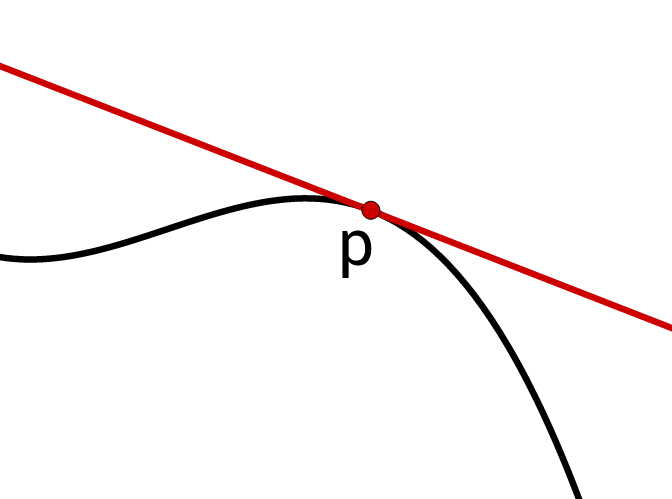
\includegraphics[scale=0.08]{curva-suave}
\end{columns}
\end{frame}

\begin{frame}
\frametitle{Ya no es suave}
\begin{columns}
\column{0.5\textwidth}

    $$\lim_{h \to 0} (f(x+h) - f(x) - f'(x) \cdot h) = 0$$

\column{0.5\textwidth}
    \begin{center}
        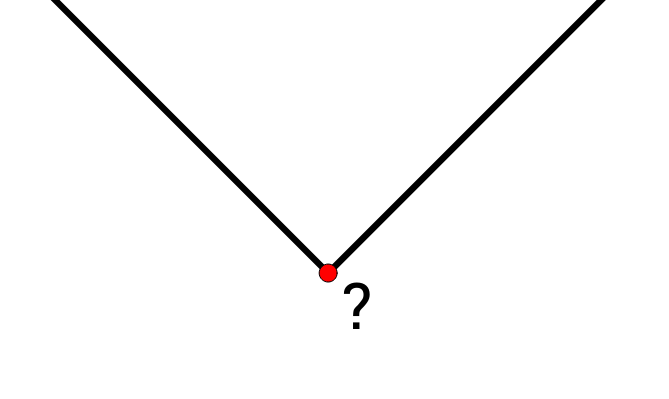
\includegraphics[scale=0.25]{curva-pico}
    \end{center}
\end{columns}
\end{frame}

\begin{frame}
  \frametitle{¿Qué buscamos?}

  \begin{block}{Preguntas clave}
    \begin{itemize}
      \item ¿Cómo determinamos el espacio tangente?
      \item ¿Qué dimensión tiene?
      \item ¿Qué relación existe entre la dimensión del espacio tangente y el espacio normal?
    \end{itemize}
  \end{block}
\end{frame}

\section{Un pequeño adelanto}

\begin{frame}
\frametitle{En general}

    Sea $f:\realR^{n} \mapsto \realR^{m}$, tenemos que

    $$\lim_{h \to 0} \| f(x+h) - f(x) - T(x) \cdot h \| = 0$$

    Cuando $f$ es diferenciable, el espacio tangente está bien determinado y es un espacio vectorial de dimensión $n$.



\end{frame}

\section{pronto ...}
\begin{frame}
\frametitle{pronto ...}

\end{frame}

\section{pronto ...}
\begin{frame}
\frametitle{pronto ...}

\end{frame}

\end{document}
